\noindent Ta có thể thực hiện một thí nghiệm quang học đơn giản bằng cách sử dụng camera của điện thoại thông minh. Camera điện thoại là một hệ gồm nhiều thấu kính, sau khi lắp ráp chỉ dày khoảng vài milimet nhờ đó có thể lắp đặt trong các chiếc điện thoại có độ dày chưa đến một centimet. Cảm biến hình ảnh của camera ghi lại hình ảnh của vật thể dưới dạng các điểm ảnh, sau đó sử dụng một phần mềm phân tích để xác định kính thước thực của ảnh. Trong các câu hỏi sau, xem camera điện thoại như một hệ thấu kính đồng trục lý tưởng được gắn cố định, ta có thể chứng minh rằng mối quan hệ giữa vật và ảnh cho bởi hệ thấu kính này tương tự với một thấu kính hội tụ và có thể sử dụng công thức thấu kính mỏng để thực hiện các tính toán liên quan. Khác với thấu kính mỏng, ta cần xác định các điểm $H$ và $H'$ (được gọi là các điểm chính) nằm trên quang trục làm điểm tham chiếu để xác định khoảng cách của vật, khoảng cách của ảnh và tiêu cự như được chỉ ra trong hình 1. Tất cả các tia sáng trong câu hỏi này đều thoả mãn điều kiện bàng trục.\\

\begin{figure}[h]
  \centering
  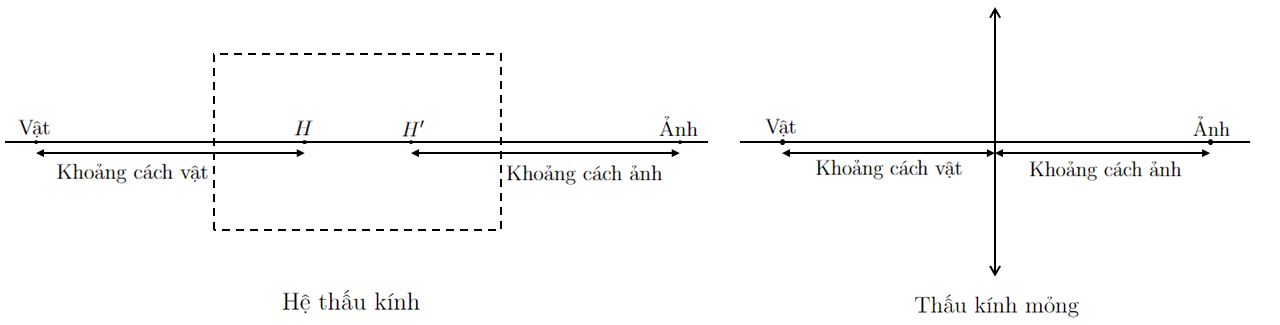
\includegraphics[width=1\textwidth]{images/Hinh 1.PNG}
  \begin{center}
    \figurename{ 1: Quan hệ vật - ảnh của hệ thấu kính và thấu kính mỏng}
  \end{center}
\end{figure}

\vspace{-20px}
\begin{enumerate}
  \item Khi ta dùng điện thoại để chụp một vật thể, do hệ thấu kính được lắp đặt bên trong điện thoại nên không thể xác định trực tiếp vị trí của điểm chính khi không biết cấu trúc và thông số của ống kính, dẫn đến không thể đo trực tiếp khoảng cách vật bằng thước. Trong thí nghiệm này, ban đầu ta đặt một nguồn sáng điểm cách trục chính một khoảng $l$, sau đó di chuyển nó dọc theo trục chính, tại các khoảng cách vật $u_{1}$ và $u_{2}$, nguồn sáng này lần lượt cho ra các ảnh nằm cách trục chính một khoảng $l_{1}$ và $l_{2}$. Gọi $s=u_{2}-u_{1}$ là độ dịch chuyển của vật trên phương trục chính. Hãy tính:
        \begin{enumerate}
          \item[a.] Tiêu cự tương đương $F$ của camera theo $l, l_{1}, l_{2}$ và $s$;
          \item[b.] Khoảng cách vật $u_{1}$ theo $l, l_{1}, l_{2}$ và $s$.
        \end{enumerate}
  \item Giả sử hệ thấu kính được sử dụng bao gồm hai thấu kính hội tụ mỏng đồng trục có tiêu cự lần lượt là $f_{1}$, $f_{2}$ và quang tâm $O_{1}$, $O_{2}$ tương ứng được đặt cách nhau một khoảng $d$. Ánh sáng xuất phát từ vật (thật hay ảo) sẽ lần lượt đi qua thấu kính $O_{1}$ và $O_{2}$ để tạo ảnh, hệ thấu kính tồn tại một mặt phẳng vật và một mặt phẳng ảnh có độ phóng đại ngang là $1$ (chúng được gọi là các mặt phẳng chính), giao điểm của các mặt phẳng này với quang trục lần lượt là điểm vật chính $H$ và điểm ảnh chính $H'$.
        \begin{enumerate}
          \item[a.] Hãy coi $H$ là vật của thấu kính $O_{1}$, tính khoảng cách vật của $H$ so với $O_{1}$. Coi $H'$ là ảnh của thấu kính $O_{2}$, tính khoảng cách ảnh của $H'$ so với $O_{2}$;
          \item[b.] Trong quá trình tạo ảnh qua hệ thấu kính, khoảng cách vật và tiêu cự vật được tính từ điểm vật chính $H$, khoảng cách ảnh và tiêu cự ảnh được tính từ điểm ảnh chính $H'$. Hãy tính tiêu cự vật $F$ và tiêu cự ảnh $F'$.
        \end{enumerate}
\end{enumerate}

